\section{Real World Languages}
\label{sec:real}

In the introduction, we stated that the original motivation behind
developing this embedding was in order to formally specify a
coarse-grained information flow control language for JavaScript.
%
In Section~\ref{sec:retrofit}, however, we used only a simplified
language as an example target language.
%
In this section, we consider the application of our embedding to
JavaScript, and two other real world target languages, Haskell, and C.
%
Our goal is to show the flexibility of the embedding in settings with
vastly different features and properties, as well as discuss the
semantic gap that must be overcome in some cases to apply our formalism
to other systems.
%
%% Two of the systems we describe have been implemented: the Haskell
%% system~\cite{lio} and the SWAPI~\cite{swapi} system; we leave the
%% implementation of the IFC system for C to future work.



\subsection{JavaScript}
\label{sec:real:js}

JavaScript, as specified by
ECMAScript~\cite{ecma}, does not have any built-in
functionality for I/O
(we denote this language as |targetLangJS|).
%
When JavaScript is embedded in web browser engines such as
Gecko or Blink, or in server-side platforms such as Node.js, additional
APIs such as the Document Object Model (DOM) or the file system
get exposed as part of the runtime system.
%
In a similar manner, we can directly implement the embedded language
|specLangJS roundrobinf| by exposing (only) our IFC primitives as part
of the runtime and running multiple instances of the JavaScript VM in
separate OS-level threads.\footnote{
  We, indeed, do this for the Gecko implementation when considering
  Web Workers that run operate OS threads.
}
%
Unfortunately, this becomes very costly when an application relies on
many tasks.
%
(Consider, for instance, a server-side web application that wishes to
create a new task for each HTTP request.)

However, this issue of performance and JavaScript isolation is not
unique to our work. 
%
In particular, browser layout engines rely on the isolation of content
from different origins (e.g., two iframes of different origins) to
implement the \emph{same-origin policy}.
%
Since creating an OS thread for each iframe is expensive, both V8 and
SpiderMonkey provide a means for running JavaScript code in isolation,
on disjoint sub-heaps of the same OS thread.
%
In V8, this unit of isolation is called a \emph{context}~\tocite{}, in
SpiderMonkey, it called a \emph{compartment}~\tocite{}.
%
Each context/compartment is associated with a global object, which, by
default, implements the JavaScript standard library (e.g.,
\verb|Object|, \verb|Array|, etc.).
%
(Gecko and Node.js expose features such as the DOM and
filesystem by extending this global object.)
%

\subsubsection{Server-side embedding for Node.js}

Using contexts as the unit of isolation, we implemented
|specLangJS seqf| for Node.js.
%
Our implementation provides a library for creating new tasks, i.e.,
contexts whose global object only contains the standard JavaScript
library and our IFC primitives (|send|, |sandbox|, etc.).
%
In turn, these tasks can create new tasks with |sandbox|.
%
Formally, |sandbox| is defined with |klone(tS) = tS0|, where |tS0| is
the global object corresponding to the standard JavaScript library and
our IFC primitives.
 
\begin{figure}
\centerline{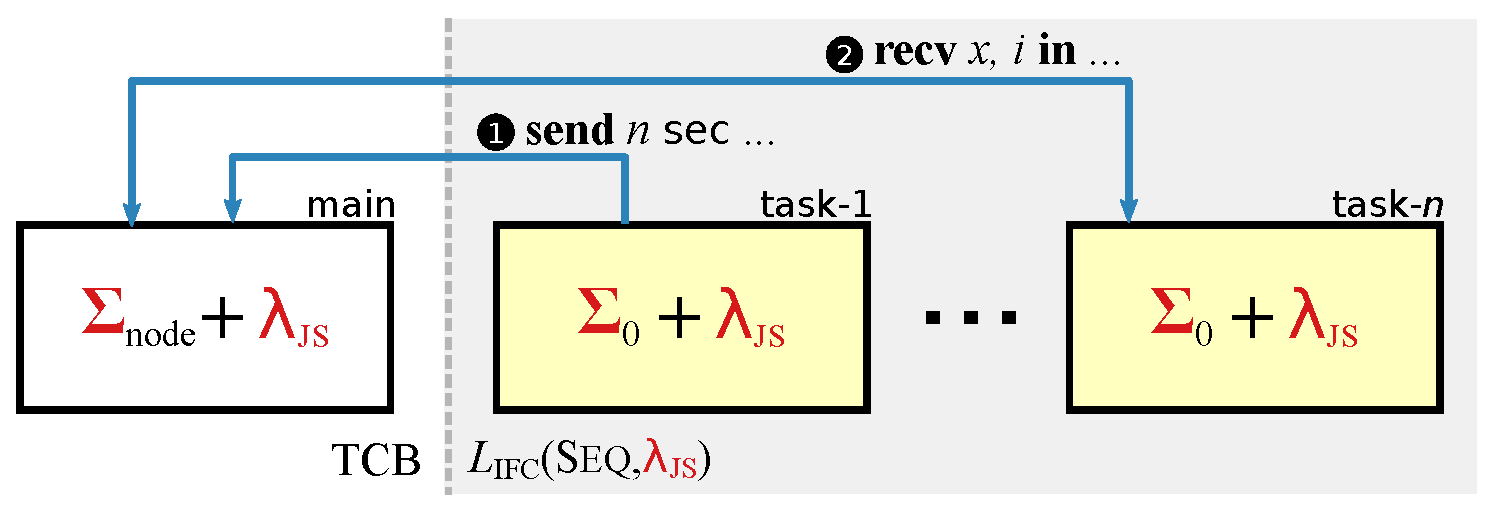
\includegraphics[width=\columnwidth]{figs/node}}
\caption{\label{fig:node} Retrofitting Node.js JavaScript with IFC.
This example shows how our trusted monitor (left) is used to mediate
communication between two tasks for which IFC is enforced(left).}
\end{figure}
As shown in Figure~\ref{fig:node}, each IFC API call from a task is mediated
by the trusted library code (the main Node.js context), that tracks
the current label, messages, etc. of each task.
%
While V8 provides a means for sharing objects between contexts that
share a security token (in the case of Blink this is used by pages of
the same origin), our API (conservatively) restricts the kinds of
messages that can be exchanged.
%
More concretely, and as mentioned in Section~\ref{sec:concrete}, we
restrict |send| (and |sandbox|) to sending string values.
%
In our formalization, this amounts to restricting the IFC language rule
for |send| such that only strings can be shared:
%{
\newcommand{\str}{"string"}
%format tOf (e) = "\texttt{typeOf}("e")\texttt{ === \str}"
%format ttrue = "\texttt{true}"
\begin{mathpar}
\inferrule[JS-send]
{
|il canFlowTo il'|\\
|iS(id') = Q|\\
|iS' = iS [ mapsto id' (il', id,  iv) , Q ]|\\
|ie = IT te|\\
|conf tS (tOf te) -> conf tS ttrue|
}
{|
iconf iS (fullconf id il tS (iniEi (send id' il' iv)), ldots)
.->
iS'; sched step (fullconf id il tS (iniEi unit), ldots)
|}
\end{mathpar}
%}
%
However, our implementation is accompanied by a library that provides
a more flexible standard library, which, among other things,
automatically marshalls JSON objects to/from strings on each
|send|/|recv|.


\Red{HERE}

We remark that this is similar to the existing
\texttt{postMessage} API used for iframe and worker
communications~\cite{webworkers}.
%
Thus, the SWAPI implementation provides an IFC version of
\texttt{postMessage}, defined in terms of |send|, that additionally
takes a label argument.

%
In turn, each task created with |sandbox| is
executed in a separate thread, running a separate, \emph{fresh} instance of our
modified JS runtime.
%
Formally, |sandbox| is defined with |klone(tS) =
tS0|, where |tS0| is the global object corresponding to the standard
JS library (e.g., |tS0| contains \texttt{Object}, \texttt{Array},
etc.).



Unsurprisingly, our coarse-grained combined language approach has been
inspired by existing browser (security) architectures.
%
Browsers, for example, isolate pages of different origins by running
them in separate runtimes.
%
Similarly, they provide the worker JS object~\cite{webworkers}, which allows
JavaScript to execute code in separate threads with separate JS
runtimes (and fresh global objects).
%
In both cases, code relies on the \texttt{postMessage} message-passing
API for communication, similar to our system.\footnote{
  The message-passing approach is, in part, due to ECMAScript's lack
  of well-defined semantics for concurrency.
  %
  Hence sharing and accessing objects such as the DOM across worker
  threads is undefined.
}
%
As suggested by our formal semantics, SWAPI can directly leverage these
mechanisms to implement the semantics of |specLangJS roundrobinf|
without modifying the JS runtime or intrusively changing the browser
layout engine.

However, a simple implementation of just associating a label with
workers and browsing context (iframes and top-level pages) to enforce
IFC on the executing JavaScript is not sufficient, as APIs which
introduce extra computational effects must be manually made aware of information flow
control.
%
For example, the initial global object of a worker contains the
\texttt{XMLHttpRequest} (XHR) object, while the global object of a
browsing context additionally contains the DOM.
%
In both cases, JS code can trivially leak information (e.g., to the
network with XHR or persistent storage using the DOM).
%
To address this, SWAPI additionally uses content security policy (CSP) and
(iframe) sandboxes~\cite{csp1.1,html5} to restrict external effects according
to the label of a task (worker or browsing context).  Accommodating these
features lies outside the purview of our formalism.

%% \Red{
%% EZY:  This seems like useless detail about the SWAPI implementation
%% that is not relevant to this paper.
%% 
%% Of course, simply disallowing all external effects for all browsing
%% contexts would break most of the Web.
%% %
%% Hence SWAPI only enforces IFC, and thus restricts external effects,
%% when the JS code uses the new API.\footnote{
%%   Once a piece of code ``opts-in'' to use our IFC API, in addition to
%%   restricting external effects we interpose ``standard''
%%   \texttt{postMessage} communication to ensure that no information is
%%   leaked between contexts that have opted-in and those that have not.
%% }
%% %
%% Moreover, rather than disallowing all external effects, SWAPI allows
%% controlled network communication by leveraging the fact that web
%% pages already have an accompanying security policy: the same origin
%% policy.
%% %
%% Hence, for example, a worker that has read data only sensitive to
%% \texttt{http://bank.ch} can communicate with this domain; only once
%% \texttt{http://aws.com} data is also included in the context will all
%% network requests be blocked.
%% %
%% Of course, this requires that we use a concrete label format to
%% express the policies; we refer the interested reader to~\tocite{} for
%% more details.}


\subsection{Haskell}
\label{sec:real:hs}
In contrast with the C embedding which relies on hardware protection
mechanisms, a Haskell implementation can leverage Haskell's strong data
abstraction and static type system, monadic approach to effects, and
lightweight concurrency to implement the embedding in a more lightweight
manner.  We briefly describe one such system, LIO~\cite{lio}, which
implements IFC as a library.

LIO is implemented by defining a new monad, \verb|LIO|, which wraps Haskell's \verb|IO|
monad.
%
The purpose of this monad is twofold: it restricts the use of
arbitrary effects that would ordinarily be allowed by the \verb|IO| monad,
and it associates labels with tasks.
%
Computations in the \verb|LIO|
monad can be thought to be operating within the IFC system.
%
One important aspect of using \verb|IO| as the base for this
implementation is that it allows use of Haskell's efficient
implementation of threads, channels, etc. (e.g., in the concurrent
version of LIO, we use Haskell's \texttt{forkIO} to fork a lightweight
thread in the case of |fork|~\cite{stefan:addressing-covert}), in
contrast to defining them in a completely pure fashion (as suggested
in Section~\ref{sec:monad}).

What is the interpretation of this system as per Section~\ref{sec:retrofit}?
%
Here, the \emph{pure subset} of Haskell is the target language, while
the monadic subset of Haskell in the \verb|LIO| monad is the IFC
language.
%
Crucially, the lack of unrestricted mutation in the pure fragment of
Haskell prevents direct communication between tasks, even when memory is
shared between them.\footnote{However, lazy evaluation can still produce
a covert channel.}

Since this IFC system is implemented as a library in Haskell,
implementation-wise, we must ensure that these languages are indeed the subsets of Haskell
we claim, i.e., while the concrete language is all of Haskell, we must
ensure that we can restrict programs to our subset of Haskell that
encodes the combined language.
%
To this end, \verb|LIO| relies on Haskell's strong data abstraction and type system
(as enforced by Safe Haskell~\cite{Terei:2012:SH:2364506.2364524}) to
ensure that arbitrary \verb|IO| actions cannot be lifted into
\verb|LIO|.
%
In other words, assuming \verb|LIO| is implemented correctly, programs
written in the \verb|LIO| monad cannot perform arbitrary \verb|IO| actions
without breaking abstraction.

We refer the interested reader to~\cite{lio,stefan:addressing-covert} for
additional details on the various implementations of this system.\footnote{It's worth noting that the proofs of non-interference we have given for asynchronous communication primitives are new and not in the original presentation of LIO.}


\subsection{C}
\label{sec:real:c}
%
C programs are able to execute arbitrary (machine) code, access
arbitrary memory, and perform arbitrary syscalls.
%
Thus, the confinement of C programs must be imposed by the underlying OS
and hardware.
%
For instance, this isolation can be achieved using Dune's hardware protection
mechanisms~\cite{Belay:2012:DSU:2387880.2387913}, similar to a simpler
version of Wedge~\cite{Belay:2012:DSU:2387880.2387913,
Bittau:2008:WSA:1387589.1387611} with an information flow control
policy.
%
Using page tables, a (trusted) IFC runtime could ensure that each task,
implemented as a lightweight process, can only access the memory it
allocates--tasks do not have access to any shared memory.
%
In addition, ring protection could be used to intercept syscalls performed by
a task and only permit those corresponding to our IFC language (such as
|getLabel| or |send|).
%
Dunes hardware protection mechanism allows us to provide a concrete
implementation that is efficient and relatively simple to reason
about, but other sandboxing mechanisms could be used in place of Dune.

In this setting, the combined language of Section~\ref{sec:retrofit}
can be interpreted in the following way: calling from the target
language to the IFC language corresponds to invoking a syscall.
%
Creating a new task with the |sandbox| syscall corresponds to
\emph{forking} a process.  Here, page tables limit what memory
a task can access: we can ensure there will be no memory (effectively
defining |klone(tS)
= tS0|, where |tS0| is the set of pages necessary to bootstrap a
lightweight process.)
%
Similarly, control over page tables and protection bits allows us to
define a |send| syscall that copies pages to our
(trusted) runtime queue; and, correspondingly, a |recv| that copies
the pages from the runtime queue to the (untrusted) receiver.
%
Since C is not memory safe, conditions on these syscalls are
meaningless.
